\begin{frame}
    \titlepage
\end{frame}



\begin{frame}
    \frametitle{Introduzione  alle Botnet}
    \begin{definition}[Botnet]
        Rete di host compromessi chiamati bot, che eseguono istruzioni impartite da un host detto botmaster, attraverso l'ausilio di un server che funge da tramite,  detto Command And Control Server (C\&C).
    \end{definition}
    \centering
    \textbf{Definita da:}
    \begin{columns}[t]

        \begin{column}{0.5\textwidth}
            \begin{itemize}
                \item Schema di comunicazione:
                      \begin{itemize}
                          \item propagazione
                                \begin{itemize}
                                    \item attiva
                                    \item passiva
                                \end{itemize}
                          \item operazione
                      \end{itemize}
                \item Topologia
                      \begin{itemize}
                          \item Centralizzata
                          \item Decentralizzata (P2P)
                          \item Ibrida
                      \end{itemize}
            \end{itemize}
        \end{column}
        \begin{column}{0.5\textwidth}
            \begin{itemize}
                \item Tecniche di occultamento/offuscamento
                      \begin{itemize}
                          \item Crittografia
                          \item Fast-flux network
                          \item Protocol Encapsulation
                          \item Stepping stones
                          \item Rootkit
                          \item Etc.
                      \end{itemize}

                \item Protocolli utilizzati
                      \begin{itemize}
                          \item HTTP, IRC, SMTP, etc.
                      \end{itemize}

            \end{itemize}
        \end{column}
    \end{columns}

\end{frame}

\begin{frame}
    \frametitle{Realizzazione dell'infrastruttura di testing}
    \begin{columns}
        \begin{column}{0.4\textwidth}
            \textbf{Tecnologie analizzate:}
            \begin{itemize}
                \item Server VMWare ESXi
                \item Firewall
                      \begin{itemize}
                          \item Netfilter
                          \item Iptables
                          \item NFtables
                          \item Firewalld
                      \end{itemize}
                \item Docker
            \end{itemize}
        \end{column}
        \begin{column}{0.6\textwidth}
            \begin{figure}
                \centering
                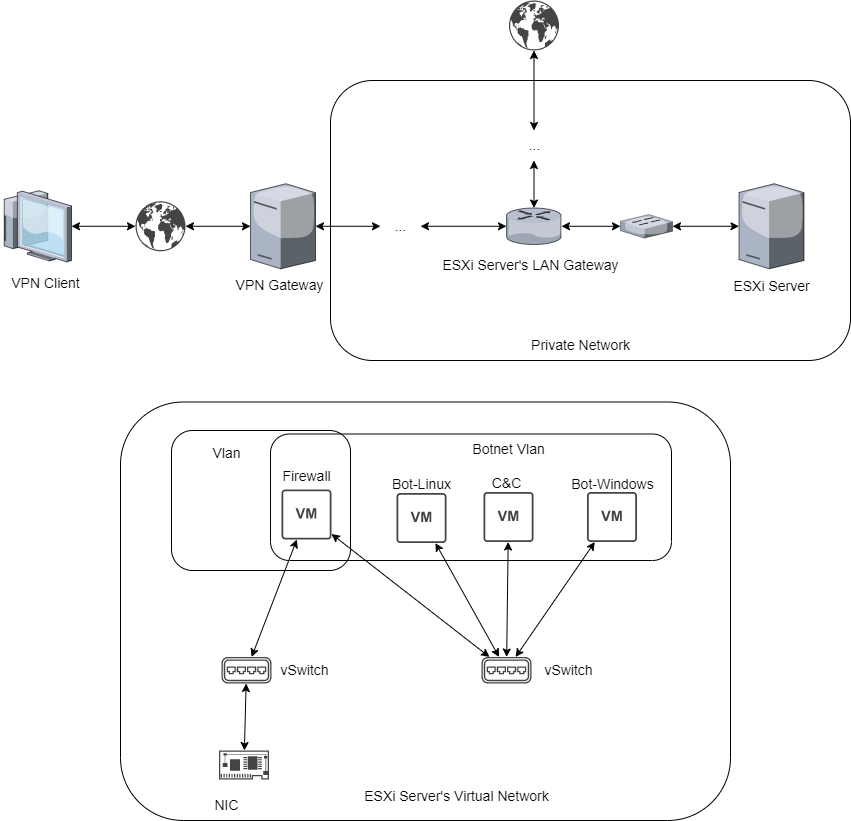
\includegraphics[width=\textwidth]{res/fig/infrastruttura1.png}
            \end{figure}
        \end{column}
    \end{columns}
\end{frame}

\begin{frame}
    \frametitle{Intrusion Detection System (IDS)}
    \begin{figure}[hbtp]
        \begin{center}
            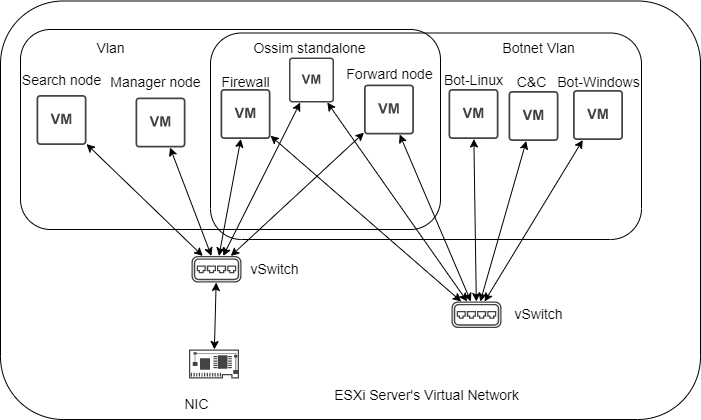
\includegraphics[width=0.6\textwidth]{res/fig/infrastruttura2.png}
        \end{center}
    \end{figure}
    \begin{columns}[t]
        \begin{column}{0.48\textwidth}
            \textbf{Categorizzabili in:}
            \begin{itemize}
                \item Signature based (SIDS)
                \item Anomaly based (AIDS)
            \end{itemize}
            oppure in:
            \begin{itemize}
                \item Network based (NIDS)
                \item Host based (HIDS)
            \end{itemize}
        \end{column}
        \begin{column}{0.48\textwidth}
            \textbf{Analizzati e utilizzati:}
            \begin{itemize}
                \item Security Onion
                \item Ossim
            \end{itemize}
        \end{column}
    \end{columns}




\end{frame}
\begin{frame}
    \frametitle{Dettagli implementativi}
    \begin{columns}[t]
        \centering
        \begin{column}{0.45\textwidth}
            \textbf{Security Onion}
            \begin{itemize}
                \item SaltStack
                \item Docker
                \item ElasticStack
                \item Vasta gamma di componenti software utilizzabili o integrabili per l'analisi di traffico di rete e di host
            \end{itemize}
        \end{column}
        \begin{column}{0.45\textwidth}
            \textbf{Ossim}
            \begin{itemize}
                \item Vulnerability assessment attraverso scansioni
                \item Intrusion detection attaverso tool NIDS, HIDS, e File Integrity Monitoring
                \item Behavioral Monitoring e capacità di availability monitoring
                \item Integrazione con OTX
            \end{itemize}
        \end{column}
    \end{columns}
    \bigskip
    Security Onion installato con architettura distribuita mentre Ossim installato in standalone
\end{frame}


\begin{frame}
    \frametitle{Studio della prima botnet - Byob}
    \begin{columns}[t]
        \begin{column}{0.48\textwidth}
            \textbf{Caratteristiche:}
            \begin{itemize}
                \item Topologia Centralizzata
                \item Push based
                \item Propagazione passiva
                \item Scitto in Python
                \item Diversi post exploitation module
                \item Zero dipendenze
                \item Multi-stage infection
            \end{itemize}
        \end{column}
        \begin{column}{0.48\textwidth}
            \textbf{Rilevazioni con NIDS:}
            \begin{itemize}
                \item Download di Stager e Payload
                \item Download di eseguibile generico
                \item Download di Miner (malware)
                \item Rilevazioni minori
            \end{itemize}
            \textbf{Non rilevati:}
            \begin{itemize}
                \item Moduli Python ad-hoc
                \item Comandi della reverse shell (crittografati con AES)
            \end{itemize}
        \end{column}
    \end{columns}
\end{frame}


\begin{frame}
    \frametitle{Agent-based HIDS: Wazuh}


    \begin{columns}[t]
        \begin{column}{0.5\textwidth}
            \textbf{Capacità:}
            \begin{itemize}
                \item Intrusion detection
                \item Analisi dei log
                \item File integrity monitoring
                \item Vulnerability detection
                \item Configuration assessment
                \item Incident response
            \end{itemize}
            \bigskip
            Installato in standalone con Docker e integrato con Sysmon

        \end{column}
        \begin{column}{0.5\textwidth}
            \begin{figure}[hbtp]
                \centering
                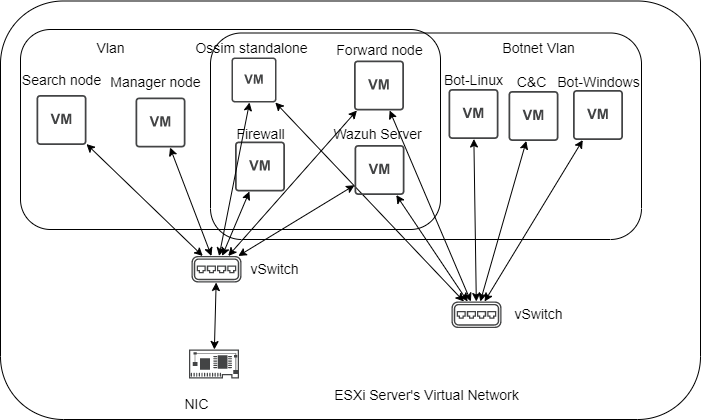
\includegraphics[width=\textwidth]{res/fig/infrastruttura3.png}
            \end{figure}
        \end{column}
    \end{columns}
\end{frame}


\begin{frame}
    \frametitle{Studio della seconda botnet - Uboat }
    \begin{columns}[t]
        \begin{column}{0.5\textwidth}
            \textbf{Caratteristiche:}
            \begin{itemize}
                \item Topologia centralizzata con possibilità di C\&C di fall-back
                \item Pull based
                \item Scritto in C++
                \item Propagazione passiva
                \item Zero dipendenze
                \item Diverse capacità operazionali
            \end{itemize}
        \end{column}
        \begin{column}{0.5\textwidth}
            \textbf{Rilevazioni con NIDS:}
            \begin{itemize}
                \item Possibilità di identificazione seppur mitigabile con comunicazioni crittografate, fast-flux network, etc.
            \end{itemize}
            \textbf{Rilevazioni con HIDS:}
            \begin{itemize}
                \item Identificazione di tutte le attività della botnet attraverso fingerprint appositamente create
            \end{itemize}

        \end{column}
    \end{columns}
\end{frame}

\begin{frame}
    \frametitle{Altri approcci SIDS analizzati}
    \begin{itemize}
        \centering
        \item Yara rules
        \item Integrazioni con virus engine
        \item API hooking
    \end{itemize}

    \medskip

    Realizzazione di prototipo basilare con l'intento di monitorare pattern di API call:
    \begin{itemize}
        \item DLL injection
        \item API hooking
        \item Generazione evento (Windows Event Log System)
        \item Collezione evento via agent
        \item Ulteriori analisi
    \end{itemize}

\end{frame}

\begin{frame}
    \frametitle{Conclusioni}
    \centering
    \textbf{Analisi approccio signature based a seguito dei test:}
    \smallskip
    \begin{columns}[t]
        \begin{column}{0.5\textwidth}
            \centering
            Pro:
            \begin{itemize}
                \item Molto efficiente nel rilevare minacce note
            \end{itemize}
        \end{column}
        \begin{column}{0.5\textwidth}
            \centering
            Contro:
            \begin{itemize}
                \item Incapace di rilevare minacce Zero Day
                \item Tipicamente rumoroso
                \item Versioning del malware e teniche di detection evasion possono rendere inefficace l'approccio
            \end{itemize}
        \end{column}
    \end{columns}

    \bigskip

    \textbf{Estensioni:}
    \begin{itemize}
        \item Approcci behavior based
        \item Automazione del deploy dell'infrastruttura
    \end{itemize}
\end{frame}

\begin{frame}
    \centering
    \Huge
    \emph{Grazie per l'attenzione}
\end{frame}